\section{Dati attività di verifica}
\subsection{Revisione dei requisti(RR)}
Al fine di presentare alla proponente i dati con la modalità a \textit{cruscotto informativo} le metriche verranno descritte attravero grafici evitando così uno stile torppo tabellare.
\subsubsection{Qualità di processo}
In questa sezione verranno analizzate le metriche e le valutazioni scaturite da esse.
\clearpage
\paragraph{Metriche dei processi}
\hspace{10cm} %risolvere il problema perchè uso il subparagraph
\newline Verranno presentate solo le metriche dei processi ISO utilizzate fino ad ora.
Per gli esiti viene usata la seguente codifica:
\begin{itemize}
	\item \textbf{X: } esito positivo;
	\item \textbf{-: } esito negativo.
\end{itemize}
\begin{table}[!htbp]
	\centering
	\renewcommand{\arraystretch}{2} 
	\rowcolors{2}{gray!25}{white}
	\begin{tabular}{|l|p{2cm}|p{7cm}|l|}
		\rowcolor{orange!50}
		\hline
		\textbf{Processo} & \textbf{Valore ottenuto} & \textbf{Commento} & \textbf{Esito} \\
		\hline
		Schedule Variance & ~~0 giorni & Come si può notare dal diagramma di gantt del \textit{piano di progetto} sono stati raggiunti gli obiettivi nei tempi prefissati. & ~~X \\
		\hline
		Budget variance & ~~\EUR{ -5} & Avendo rispettato gli obiettivi entro la deadline prestabilita non ci sono aumenti minimi. &  ~~X \\
		\hline
		{Indisponibilità servizi esterni} & ~~0 & Tutti i servizi esterni da noi usati non hanno avuto disservizi.  & ~~X\\
		\hline
		Rischi non calcolati & ~~0 & Per questa deadline non sono emerse problematiche pertanto non sono presenti rischi non calcolati che gravano sul progetto. & ~~X\\
		\hline
	\end{tabular}
	\caption{Metriche dei processi}
\end{table}
\clearpage
\paragraph{Maturità macro-processi ISO }
\hspace{15cm}
\begin{figure}[h!]
	\centering
	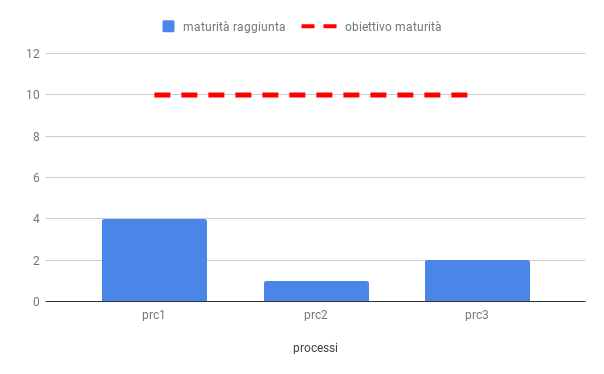
\includegraphics[scale=0.5]{MaturitaProcessi.png}
	\caption{Maturità macro-processi ISO 15504}
\end{figure}
\begin{itemize}
	\item \textbf{P1:} processo gestito da automatismi, il gruppo sta imparando ad utilizzare quest'ultimi per rendere il lavoro più preciso e con meno possibilità di errore. Usando ad esempio Toggl per il conteggio ore e integrazione slack con github tracciando le issue ha
	permesso di ottenere una migliore pianificazione;
	\item \textbf{P2:} processo non ancora istanziato poichè non fa parte della revisione di requisiti, abbiamo analizzato solo metriche in funzione degli obiettivi;
	\item \textbf{P3:} processo non ancora istanziato, sarà comunque quasi completamente automatizzato.
\end{itemize}
\clearpage
\subsubsection{Qualità di prodotto}
In questa fase ci si concentra principalmente sulla redazione dei documenti, pertanto le uniche metriche utilizzate sono quelle riguardanti i documenti.
Poichè, in particolari circostanze (non necessariamente rare), la valutazione automatica della leggibilità, se non tiene conto in alcun modo dei significati delle parole, può dare risultati inattendibili, per non dire fuorvianti si è scelto di non valutare i documenti tramite script che calcolano le metriche.
Nonostante ciò sono metriche puramente sintattiche, sono da considerare con la dovuta cautela. \\
Come si può notare dal trend dei grafici l'obiettivo è stato quasi sempre rispettato ottenendo dei documenti con una leggibilità media da istruzione superiore.
	\clearpage
\paragraph{Gunning Fog index}
\hspace{15cm}
\begin{figure}[!htbp]
	\centering
	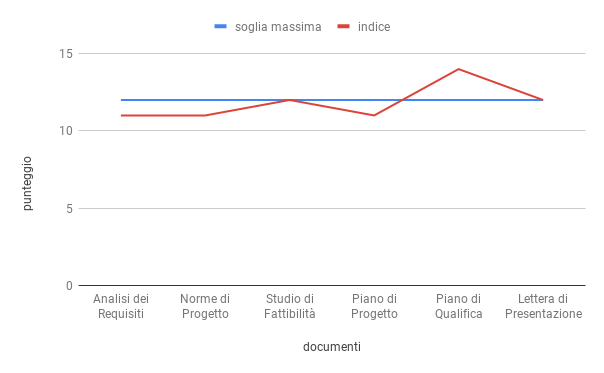
\includegraphics[scale=0.5]{GunningFogIndex.png}
	\caption{Gunning Fog index}

\end{figure}
%\clearpage
\paragraph{Simple Measure of Gobbledygook (SMOG)}
\hspace{15cm}
\begin{figure}[!htbp]
	\centering
	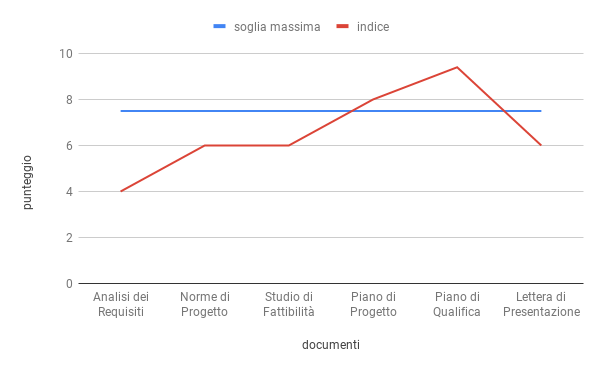
\includegraphics[scale=0.5]{Smog.png}
	\caption{SMOG}
\end{figure}
\clearpage
\paragraph{Gulpease Index}
\hspace{15cm}
\begin{figure}[!htbp]
	\centering
	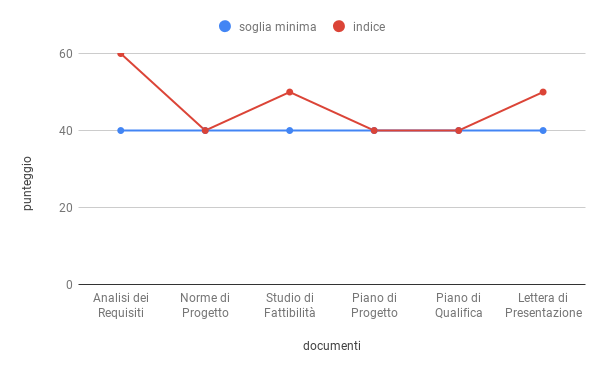
\includegraphics[scale=0.5]{GulpeaseIndex.png}
	\caption{Gulpease index}
\end{figure}

\myparagraph{Errori sintattici}
 I verificatori hanno eliminato gli errori rimanenti presenti nei documenti, raggiungendo così il valore ottimale prefissato attraverso il software per il controllo ortografico presente in TexStudio. 
 
\subsubsection{Conclusioni}
Complessivamente il gruppo non ha sforato il monte ore prestabilito ed il Budget Variance e' stato di -0.037\% che equivale ad un aumento di \EUR{5}. Tale aumento non andrà ad influenzare il costo del preventivo a termine. 
\clearpage
\subsection{Revisione di Progettazione (RP)}
Questa sezione verrà riempita durante il periodo definito.
\subsection{Revisione di Qualifica(RQ)}
Questa sezione verrà riempita durante il periodo definito
\subsection{Revisione di Accettazione(RA)}
Questa sezione verrà riempita durante il periodo definito
